\documentclass[a4paper]{article}
\usepackage{xcolor}
\usepackage{amsmath}
\usepackage{mathtools}
\usepackage{siunitx}
\usepackage{booktabs}

\title{Comparison of Terrain Following and Cut Cell Grids with a Non-Hydrostatic Model}
\author{James Shaw}
\date{TODO}

\begin{document}
\newcommand{\TODO}[1]{\textcolor{purple}{TODO: \emph{#1}}}
\newcommand{\textcite}[1]{\textbf{#1}}

\maketitle

Builds on the work of \textcite{schaer2002} (MWR), \textcite{klemp2011} (MWR), \textcite{weller-shahrokhi2014} (MWR)

Results also compared with \textcite{melvin2010} (QRJ), maybe \textcite{zaengl2012} (MWR), \textcite{good2014} (Atmos Sci Letters)

\section{Introduction}

\begin{itemize}
	\item Comparing results BTF, SLEVE and cut cell style grid for three standard two-dimensional test cases
	\item Small cell problem
\end{itemize}

\section{Results}
\begin{itemize}
	\item \TODO{How much do I need to say about the model?  Just cite \textcite{weller-shahrokhi2014}?}
	\item \TODO{Include BTF equations from \textcite{galchen-somerville1975} and SLEVE equations from \textcite{schaer2002}?}
	\item \TODO{Explain how SnapCol grid is constructed?}
\end{itemize}

\subsection{Advection}
\begin{itemize}
	\item Motivation: tests advection scheme accuracy, especially with grid distortions
	\item Specify domain, terrain, discretisation in time and space, tracer
	\item Specify wind field, projection method for non-divergence
	\item Advection equation in flux form
	\item Upwind-biased cubic advection scheme, non-monotonic, not flux corrected
	\item d/dt scheme (RK2)
\end{itemize}

We compare the following grids:
\begin{itemize}
	\item No orography (which tells us how good the model can get)
	\item BTF
	\item SLEVE (only briefly since it's not adding so much to our argument)
	\item SnapCol (briefly because it's the same as noOrography)
\end{itemize}

Analysis:
\begin{itemize}
	\item Upwind-biased cubic is qualitatively better than Sch\"ar's 4th order leapfrog on BTF grid (figure~\ref{fig:advection})
	\item SnapCol error, min and max is almost identical to noOrography (unsurprisingly) (table~\ref{tab:advection})  This agrees with \textcite{good2014}
	\item SLEVE error, min and max are part-way between BTF and noOrography (again, unsurprisingly)
	\item noOrography, BTF and SLEVE min and max comparable to \textcite{schaer2002}
	\item Conclusion: advection more accurate on more regular grids, but nevertheless satisfactory on all grids
\end{itemize}

\begin{figure}
	btf-cubicUpwindCPCFit-divFree \\
	\input{../advectTracer-horizontal-btf-cubicUpwindCPCFit-divFree/tracer-contour}
	\input{../advectTracer-horizontal-btf-cubicUpwindCPCFit-divFree/error-contour}

	schaer-4thorder \\
	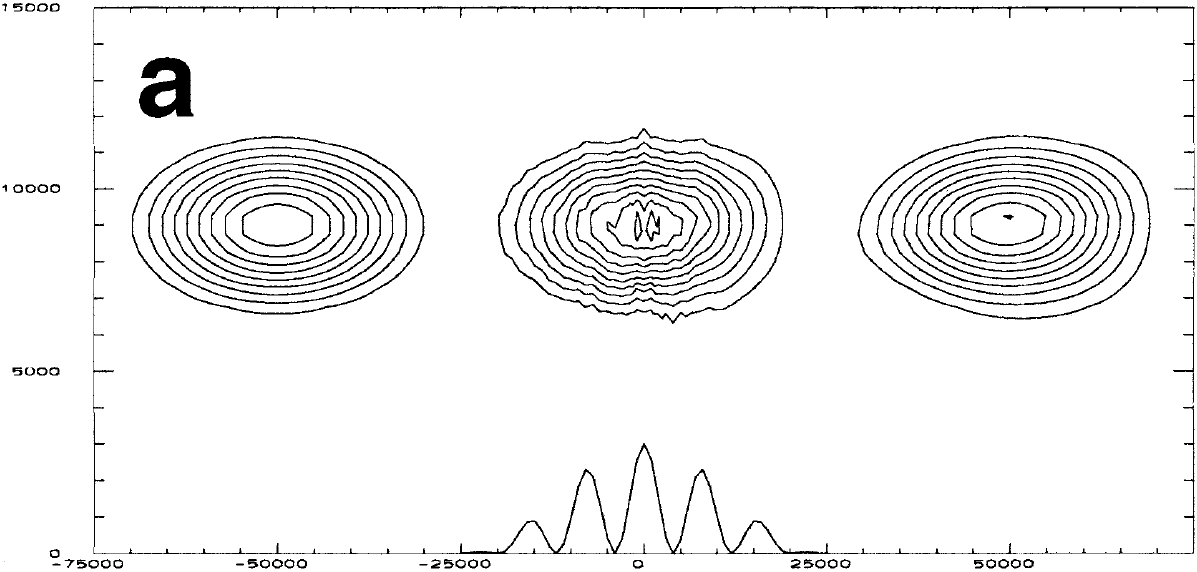
\includegraphics[height=1.5in]{schaer-btf-4thorder.png}
	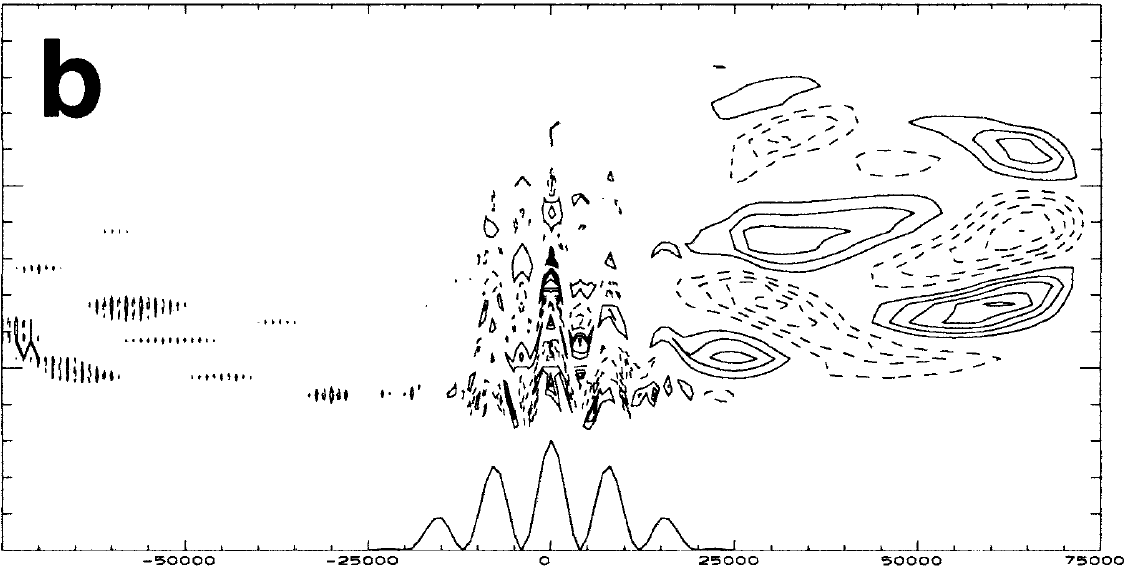
\includegraphics[height=1.5in]{schaer-btf-4thorder-error.png}
%
	\caption{Comparing our BTF cubicUpwindCPCFit result with Schaer's 4th order result}
	\label{fig:advection}
\end{figure}

\begin{table}
\centering
\begin{tabular}{ l l l l l l }
\toprule
& \multicolumn{3}{c}{Cubic upwind-biased} & \multicolumn{2}{c}{Sch\"ar 4th order} \\
& $\ell^2$ error & min & max & min & max \\
\midrule
Analytic  & 0 & 0 & 1 & \multicolumn{1}{c}{---} & \multicolumn{1}{c}{---} \\
BTF 	  & TODO & TODO & TODO & \num{-0.058} & \num{1.001} \\
SnapCol   & TODO & TODO & TODO & \multicolumn{1}{c}{---} & \multicolumn{1}{c}{---} \\
noOrography & TODO & TODO & TODO & \num{-0.002} & \num{0.984} \\
\bottomrule
\end{tabular}
%
\caption{Min, max and error norms compared with \textcite{schaer2002}}
\label{tab:advection}
\end{table}

\subsection{Resting atmosphere}

\TODO{do we want to discuss energy measures?  1. we can't compare our results with anybody else, 2. we'll have to explain how we calculate the energy measures 3. it could open a can of worms w.r.t. lack of conservation}

\begin{itemize}
	\item Motivation: challenge accuracy of H operator (\TODO{if we mention H op here we'll have to explain it beforehand})
	\item Specify domain, thermodynamics, discretisation in time and space
\end{itemize}

Analysis:
\begin{itemize}
	\item Spurious $w$ significantly less than those found by \textcite{klemp2011} for BTF: \SI{0.35}{\meter\per\second} vs \SI{10}{\meter\per\second}
	\item SnapCol $w$ (\SI{1e-3}{\meter\per\second}) significantly lower and energy conservation better than BTF or SLEVE
	\item Formulation is not energy conserving
	\item \TODO{Could also compare with \textcite{zaengl2012}, \textcite{good2014}?}
	\item Conclusion: non-orthogonality is a significant cause of numerical error in this test but, again, satisfactory on all grids
\end{itemize}

\begin{figure}
	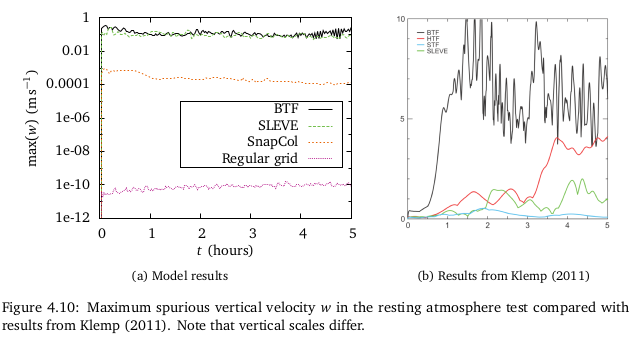
\includegraphics[height=3in]{resting-atmosphere-w.png}
%
	\caption{Comparing our results with \textcite{klemp2011}'s}
	\label{fig:resting}
\end{figure}

\subsection{Gravity waves}
\begin{itemize}
	\item \TODO{Motivation: it models a real dynamic process?}
	\item Specify domain, thermodynamics, prescribed inlet wind
	\item Specify sponge layers, BCs
	\item Compare BTF, SLEVE and SnapCol results (SLEVE only briefly as visually identical to BTF)
\end{itemize}

Analysis:
\begin{itemize}
	\item $w$ contours visually similar on all grids, agree with \textcite{melvin2010} (Figure~\ref{fig:gw-w})
	\item \TODO{don't know if divergence is relevant -- it's greater on the SnapCol grid (MSc dissertation Figure 4.15e)}
	\item $\theta$ anomalies similar on all grids EXCEPT...
	\item ... on SnapCol grid in lee of mountain near the ground. (Figure~\ref{fig:gw-theta})
	\item \TODO{worth mentioning implications of this?  1. reduced stability, although not enough to create vertical motion in this instance 2. model has no viscosity so thermal mixing should not occur in theory}
	\item Lorenz computation mode has been excited because Exner sample line at $x = \SI{50}{\kilo\meter}$ is in hydrostatic balance (Figure~\ref{fig:gw-exner-theta})
	\item \TODO{We can speculate on what excites the computational mode, but perhaps better not to?}
	\item Little/no evidence of small cell problem -- \TODO{don't know that we can say much here without another vertical momentum test; our hypothesis about the quasi-horizontal flow isn't backed up with a test case}
	\item Conclusion: results similar on all grids, agree with literature, except for Lorenz computational mode on SnapCol grid
\end{itemize}

\begin{figure}
	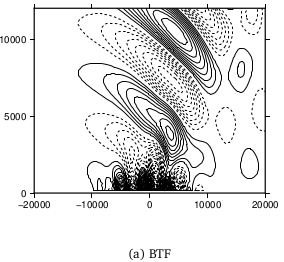
\includegraphics[height=2in]{gw-w-btf.png}
	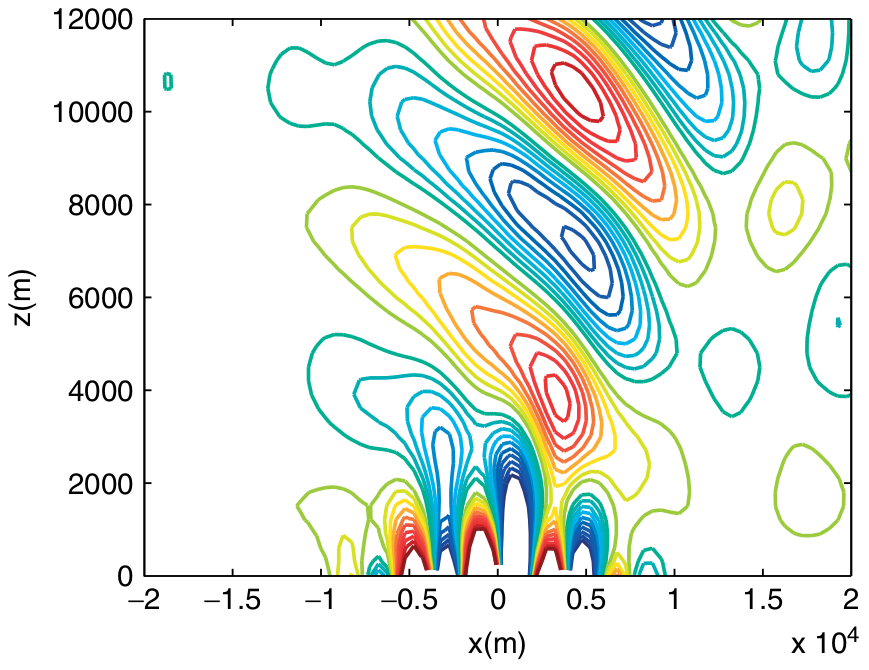
\includegraphics[height=2in]{melvin-7a.png}
%
	\caption{Gravity wave vertical velocities and thermal anomalies from initial thermal profile}
	\label{fig:gw-w}
\end{figure}

\begin{figure}
	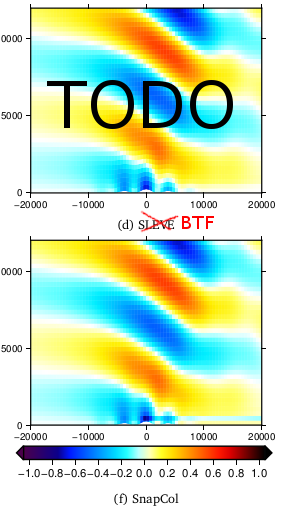
\includegraphics[height=3in]{gw-theta.png}
	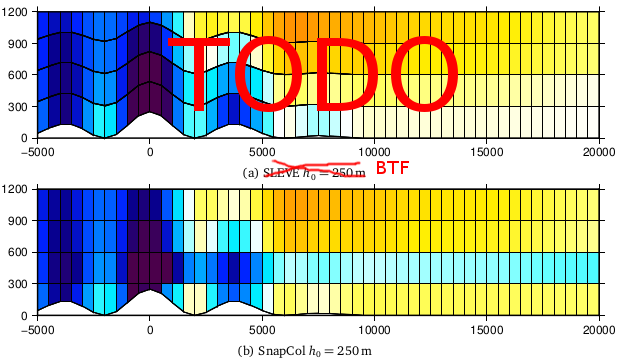
\includegraphics[height=3in]{gw-theta-zoom.png}
%
	\caption{Gravity wave thermal anomalies from initial thermal profile}
	\label{fig:gw-theta}
\end{figure}

\begin{figure}
	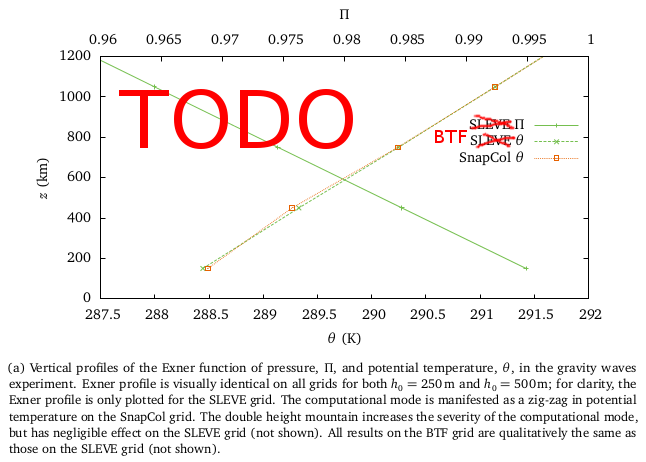
\includegraphics[height=3in]{gw-exner-theta.png}
%
	\caption{Vertical sample line of Exner function of pressure and theta to demonstrate Lorenz computational mode}
	\label{fig:gw-exner-theta}
\end{figure}


\section{Conclusions}
\begin{enumerate}
	\item BTF grid isn't as bad as people say it is.  We found that:
	\begin{itemize}
		\item Upwind-biased cubic advection scheme accurately advects a tracer in non-divergent flows (Figure~\ref{fig:advection}, Table~\ref{tab:advection})
		\item spurious vertical velocities are small in resting atmosphere (Figure~\ref{fig:resting})
		\item gravity waves results visually as good as reference solution from \textcite{melvin2010} (figure~\ref{fig:gw-w})
	\end{itemize}

	\item Cut cell grids can be worse than TF grids:
	\begin{itemize}
		\item Lorenz computational mode found on SnapCol grid only (figure~\ref{fig:gw-theta}, \ref{fig:gw-exner-theta})
	\end{itemize}

	\item Cut cell grids can also be better than TF grids in more artificial test cases:
	\begin{itemize}
		\item SnapCol $w$ two orders of magnitude smaller in resting atmosphere test
		\item SnapCol advection test as good as noOrography
	\end{itemize}
\end{enumerate}

\textbf{With the exception of the Lorenz computational mode on the SnapCol grid in the gravity waves test, results were satisfactory across BTF, SLEVE and SnapCol grids in all three test cases.}

Miscellany:
\begin{itemize}
	\item Advection accuracy depends on alignment of the flow with grid layers (\TODO{we kinda need wobblyTracerAdvection to reach this conclusion})
	\item Formulation does not conserve energy (evidenced in resting atmosphere test, Fig 4.12d in MSc dissertation)
\end{itemize}

\section{Further work}
\begin{itemize}
	\item Lorenz computational mode motivates formulation of C-P staggering for cut cell grids
	\item Find out what excites the Lorenz computational mode
\end{itemize}

\end{document}
